    \begin{figure}[H]
        \centering
        \begin{subfigure}[b]{0.45\linewidth}
            \centering
            \begin{tikzpicture}[line cap=round, line join=round, x=1cm, y=1cm]
                \clip (-0.5, 0) rectangle (5, 3.5);
                \coordinate (a) at (0.21, 0.14);
                \coordinate (b) at (0.62, 2.82);
                \coordinate (c) at (2.01, 1.32);
                \coordinate (d) at (4.23, 2.23);
                \draw (c) -- (d);
                \foreach \point/\pos in {a/above left, b/above left, c/below right, d/above right}
                    \draw[fill=black] (\point) circle (1pt) node[\pos] {$\point$};
            \end{tikzpicture}
            \caption*{$F_0 K$}
        \end{subfigure}
        \hfill
        \begin{subfigure}[b]{0.45\linewidth}
            \centering
            \begin{tikzpicture}[line cap=round, line join=round, x=1cm, y=1cm]
                \clip (-0.5, 0) rectangle (5, 3.5);
                \coordinate (a) at (0.21, 0.14);
                \coordinate (b) at (0.62, 2.82);
                \coordinate (c) at (2.01, 1.32);
                \coordinate (d) at (4.23, 2.23);
                \draw (c) -- (d) -- (b) -- cycle;
                \foreach \point/\pos in {a/above left, b/above left, c/below right, d/above right}
                    \draw[fill=black] (\point) circle (1pt) node[\pos] {$\point$};
            \end{tikzpicture}
            \caption*{$F_1 K$}
        \end{subfigure}

        \vspace{0.5cm} % Add vertical space between rows

        \begin{subfigure}[b]{0.45\linewidth}
            \centering
            \begin{tikzpicture}[line cap=round, line join=round, x=1cm, y=1cm]
                \clip (-0.5, 0) rectangle (5, 3.5);
                \coordinate (a) at (0.21, 0.14);
                \coordinate (b) at (0.62, 2.82);
                \coordinate (c) at (2.01, 1.32);
                \coordinate (d) at (4.23, 2.23);
                \coordinate (e) at (4.64, 0.91);
                \coordinate (f) at (2.78, 0.63);
                \draw (a) -- (b) -- (c) -- cycle;
                \draw (c) -- (d) -- (b);
                \foreach \point/\pos in {a/above left, b/above left, c/below right, d/above right, e/below right, f/below}
                    \draw[fill=black] (\point) circle (1pt) node[\pos] {$\point$};
            \end{tikzpicture}
            \caption*{$F_2 K$}
        \end{subfigure}
        \hfill
        \begin{subfigure}[b]{0.45\linewidth}
            \centering
            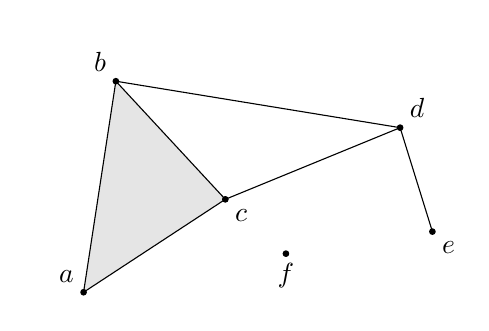
\begin{tikzpicture}[line cap=round, line join=round, x=1cm, y=1cm]
                \clip (-0.5, 0) rectangle (5, 3.5);
                \coordinate (a) at (0.21, 0.14);
                \coordinate (b) at (0.62, 2.82);
                \coordinate (c) at (2.01, 1.32);
                \coordinate (d) at (4.23, 2.23);
                \coordinate (e) at (4.64, 0.91);
                \coordinate (f) at (2.78, 0.63);
                \fill[fill=black, fill opacity=0.1] (a) -- (b) -- (c) -- cycle;
                \draw (a) -- (b) -- (c) -- cycle;
                \draw (c) -- (d) -- (b);
                \draw (d) -- (e);
                \foreach \point/\pos in {a/above left, b/above left, c/below right, d/above right, e/below right, f/below}
                    \draw[fill=black] (\point) circle (1pt) node[\pos] {$\point$};
            \end{tikzpicture}
            \caption*{$F_3 K$}
        \end{subfigure}
        \caption{Four step filtration of a simplicial complex $K$.}
        \label{fig:filtration}
    \end{figure}